\section{Parte I - Caso Base}
% En esta sección se describe el CÓMO se realizó el estudio.
% Deben describir el sistema, las herramientas y el análisis del caso inicial.

El presente estudio analiza la operación diaria de un sistema eléctrico basado en la topología IEEE de 14 barras, modelado con el ecosistema Sienna en Julia mediante los paquetes \texttt{PowerSystems.jl}, \texttt{PowerSimulations.jl} y \texttt{PowerFlows.jl}. Para el análisis del caso base, se procedió a incorporar un perfil horario de demanda normalizado, el cual incrementa la carga base del sistema en un 10\%, y se reemplazó el generador síncrono térmico de la barra 3 por una planta de generación fotovoltaica (solar) de igual capacidad máxima ($0.9$ pu en base $S_{base}=100$ MVA). A dicha planta se le asignó costo variable nulo, sin capacidad de regulación de potencia reactiva (operando a factor de potencia unitario) y se le aplicó un perfil de irradiancia solar normalizado a lo largo de un horizonte de operación de 24 horas.

\subsection{Despacho económico}

Para la determinación de los puntos óptimos de generación de las unidades en cada hora, se formuló un problema de Despacho Económico (ED) para un horizonte de 24 horas. Se empleó el modelo de red equivalente \texttt{CopperPlatePowerModel}, el cual ignora las restricciones de capacidad de transmisión de las líneas y únicamente impone el balance global entre generación y demanda, respetando los límites de potencia mínima y máxima de cada unidad. La optimización fue resuelta utilizando el solver Ipopt.

En la figura \ref{fig:despacho} se observa el aporte de potencia activa de cada unidad generadora apilado sobre la curva de demanda total del sistema.

\begin{figure}[htbp]
\centering
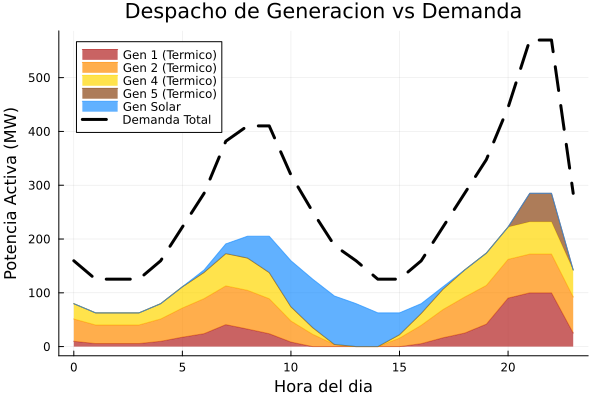
\includegraphics[width=\columnwidth]{Graficos_Resultados/1_despacho_areas.png} 
\caption{Despacho de potencia activa y perfil de demanda total del sistema durante 24 horas.}
\label{fig:despacho}
\end{figure}

El impacto de considerar la planta fotovoltaica dentro del mix de generación es evidente durante las horas diurnas. Dado que la energía solar tiene costo variable nulo, el optimizador la despacha con prioridad máxima. En las horas de mayor irradiancia (13:00 y 14:00 hrs), la planta solar logra abastecer el 100\% de la demanda del sistema, desplazando por completo al parque generador térmico y minimizando el costo de operación. 

Esta priorización tiene un impacto directo en el costo marginal de la energía ($\lambda$) del sistema, el cual refleja el costo de proveer un MW adicional, tal como se presenta en la figura \ref{fig:costo_marginal}.

\begin{figure}[htbp]
\centering
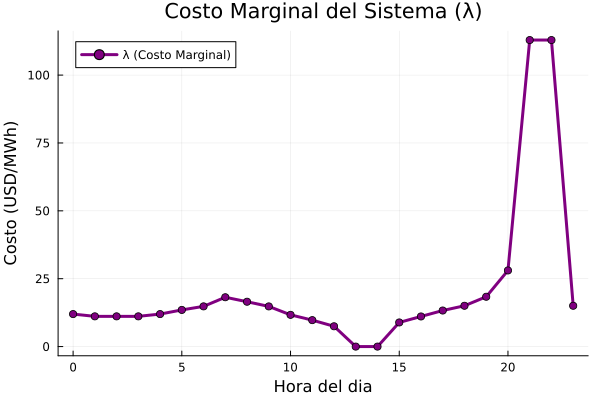
\includegraphics[width=\columnwidth]{Graficos_Resultados/2_costo_marginal.png} 
\caption{Evolución del costo marginal del sistema ($\lambda$) en USD/MWh.}
\label{fig:costo_marginal}
\end{figure}

Durante las horas solares, el $\lambda$ colapsa a valores cercanos a cero ($0$ USD/MWh). Por el contrario, a las 21:00 y 22:00 hrs ocurre la mayor exigencia del sistema: la demanda alcanza su máximo (284.9 MW) justo cuando la inyección solar es nula. Para satisfacer esta carga, se agota la capacidad de los generadores más económicos (gen-1, gen-2 y gen-4) forzando el encendido del generador más costoso de la red, gen-5. Como la función de costo de dicha unidad es cuadrática, la derivada determina su respectivo costo marginal:

\begin{equation}
\lambda = \frac{dC_5}{dP_5} = 60 + P_5
\label{eq:lambda}
\end{equation}

Al despachar el gen-5 con $P_5 = 52.9$ MW para cubrir el déficit nocturno, la ecuación \eqref{eq:lambda} dictamina que el costo marginal del sistema asciende abruptamente a 112.9 USD/MWh, explicando el salto extremo observable en la figura \ref{fig:costo_marginal}.

\subsection{Flujo de potencia}

Con los setpoints de potencia activa resultantes del Despacho Económico, se procedió a ejecutar 24 flujos de potencia AC (uno para cada hora) con el objetivo de evaluar la operación real de la red, incluyendo la respuesta de potencia reactiva de las unidades sincrónicas. Para ello, se configuró el solver habilitando la verificación de límites de potencia reactiva (\texttt{check\_reactive\_power\_limits=true}).

A partir de los resultados de flujo de potencia, se extrajo el perfil de tensiones para todos los nodos del sistema. En particular, la figura \ref{fig:voltajes} muestra la evolución de la magnitud de tensión para las cuatro barras que presentaron las mayores caídas a lo largo del día.

\begin{figure}[htbp]
\centering
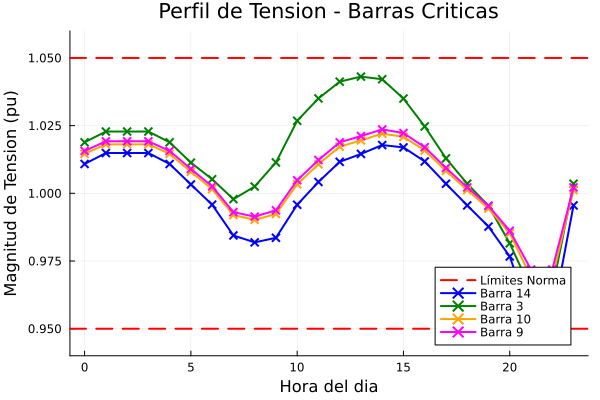
\includegraphics[width=\columnwidth]{Graficos_Resultados/3_perfiles_tension_criticos.png} 
\caption{Evolución horaria de la magnitud de tensión (pu) para las barras más críticas del sistema.}
\label{fig:voltajes}
\end{figure}

Al analizar los resultados, se constata que las magnitudes de voltaje de todas las barras de la red se mantienen íntegramente dentro de los límites operativos exigidos por la norma técnica, sin sobrepasar el límite superior ni caer por debajo del umbral mínimo de seguridad ($0.95 \text{ pu} \leq |V| \leq 1.05 \text{ pu}$). El sistema, sustentado por la capacidad de inyección y absorción de reactivos de los generadores síncronos restantes, posee la robustez necesaria para soportar los grandes cambios de flujos de potencia activa inducidos por la intermitencia fotovoltaica sin comprometer la estabilidad del voltaje local.
